\documentclass[presentation]{beamer}
\usepackage{oop-slides}
\usepackage{ragged2e}
\usepackage{cleveref}
\setbeamertemplate{bibliography item}[text]
\newcommand{\lessonnr}[0]{06}
\title[OOP07 -- Advanced]{07 \\ Decentralized Version Control Systems, \\ Eccezioni e Reflection}
\newcommand{\ditto}{\texttt{\char`\"}}

\addtobeamertemplate{block begin}{}{\justifying}
\addtobeamertemplate{frame begin}{}{\justifying}

\begin{document}

\frame[label=coverpage]{\titlepage}

%====================
%Outline
%====================
% \fr{Outline}{
%   \bl{Goal della lezione}{
%     \iz{ 
% 			\item Sviluppo sinergico di codice in team
% 				\iz{
% 					\item Principi di base dei moderni sistemi di versioning
% 					\item Utilizzo locale di un Distributed Versions Control System
% 					\item Mercurial come esempio di DVCS
% 					\item Bitbucket come esempio di servizio per repository hosting
% 					\item Workflow suggeriti per lo sviluppo di progetti software
% 				}
% 			\item Definizione ed uso di nested class (quando necessario)
% 			\item Uso della Java Reflection API
% 			\item Definizione ed uso di enumerazioni (enum)
% 	  }
% 	}
% }

\begin{frame}<beamer>
 	\frametitle{Outline}
 	\tableofcontents[]
\end{frame}

\section{Decentralized version control systems I}

\subsection{Generalità}

\fr{Cosa sono}{
   I DVCS sono software che consentono di:
   \iz{
      \item Mantenere traccia dei cambiamenti fatti ad un progetto, consentendo di andare ``avanti e indietro'' nel tempo.
      \item Consentire e promuovere il lavoro di gruppo, anche in parallelo (lo vedremo nel prossimo lab)
   }

	L'esigenza di poter tornare a salvataggi precedenti è sempre stata avvertita dagli sviluppatori (e non solo). L'operazione di salvare più stati del proprio lavoro è detta \textit{versioning}, un software che semplifica il versioning è un \textit{version control system} (o \textit{versioning system}).
}

\fr{Pillole di storia}{

	Sistemi di versioning:
	\iz {
		\item ``Fai da te'' --- è il sistema che la maggior parte di voi ha usato finora: si fa una copia di tutti i file in una cartella (magari numerata). Costa molto in spazio ed in tempo, rende difficile lo scambio di file e il lavoro parallelo.
		\item \emph{CVS} --- Fu il primo sistema di versioning. Studiato per salvare automaticamente i punti di salvataggio di file di testo. È difficile usarlo per file binari, facilita lo scambio di file rispetto ad inviarsi cartelle.
		\item \emph{SVN} --- Evoluzione di CVS. Molto più veloce e con supporto nativo a file binari. Il lavoro in parallelo è possibile a patto di adottare un flusso di lavoro di squadra molto controllato.
		\item \emph{Git} e \emph{Mercurial} --- Sviluppati parallelamente per superare le limitazioni di SVN, sono nati praticamente identici. Più veloci di SVN e pensati per supportare il lavoro massivamente parallelo di team sparsi per il mondo.
	}
}

\fr{Diffusione}{
   Sono usati per (quasi) tutti i moderni processi di sviluppo software. Un po' di esempi:
   \iz{
      \item Android (git)
      \item Drupal (git)
      \item Facebook (Mercurial)
      \item GCC (git)
      \item Go (Mercurial)
      \item Java JDK (Mercurial)
      \item Libreoffice (git)
      \item Linux kernel (git)
      \item Nokia Maps (Mercurial)
      \item Python (Mercurial)
      \item VLC Video Player (git)
      \item Wine (git)
      \item le slides del prof. Viroli (Mercurial)
      \item le slides e le esercitazioni di laboratorio di OOP! (git)
   }
}

\fr{Diffusione}{
	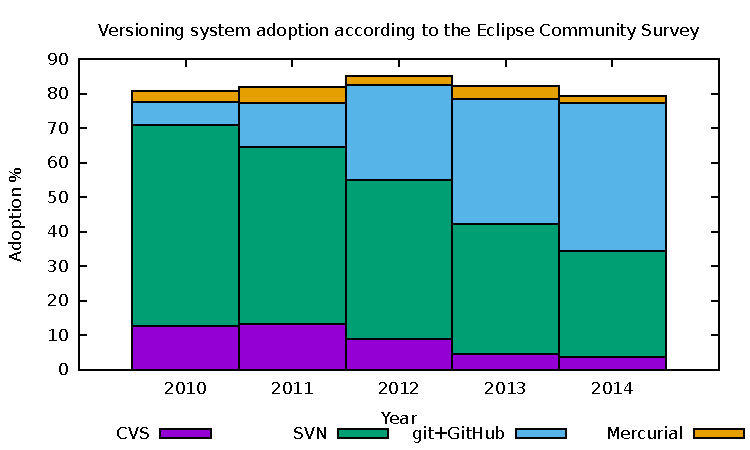
\includegraphics[width=\textwidth]{img/chart}
}

\begin{frame}{Parentesi: perché Mercurial}
	Dalla slide precedente si vede che non è il più diffuso, né quello in più rapida espansione. Perché non git?
	\begin{itemize}
		\item Nasconde le feature avanzate
		\item Didatticamente più semplice
		\item Identici principi di base
		\item Spesso identici comandi
		\item git richiede una shell Unix per funzionare, e su Windows questa va emulata tramite Cygwin
		\item Molto più Windows friendly, e purtroppo:
		\begin{itemize}
			\item Sui PC del laboratorio abbiamo Windows
			\item Molti studenti lo usano anche per sviluppare
		\end{itemize}
	\end{itemize}
	Se il trend continuasse e il dominio di git diventasse ancor più marcato, è possibile che in futuro insegneremo direttamente git.
	
	Chi ha capito bene Mercurial, imparerà git in un paio d'ore.
\end{frame}

\subsection{Concetti fondamentali}

\fr{Concetti basilari}{
  \bl{Repository}{
    Il repository è l'insieme dei file che vengono tracciati dal DVCS assieme ai metadati, ossia alle informazioni che servono a ricostruire qualunque stato precedente.
  }
  \bl{Tracking differenziale}{
    Il tracking differenziale è l'abilità di registrare le differenze fra diverse versioni di uno o più file. Invece di salvare l'intero stato (tutto il contenuto di un file), vengono salvate solo le informazioni necessarie a ricostruire il file a partire dal salvataggio precedente.
  }
  \bl{Navigazione della history}{
		La navigazione della history è la possibilità di far tornare uno qualunque dei file del repository ad uno qualunque dei salvataggi precedenti (o successivi, se ce ne sono).
  }
}

\fr{Flussi di lavoro}{
  \bl{Branching} {
		Il branching è l'abilità di avviare nuove linee di lavoro a partire da un salvataggio precedente.
  }
  \bl{Merging} {
		Il merging è l'abilità di unire linee di lavoro separate in una unica.
  }
	\vspace{1cm}
	\centering 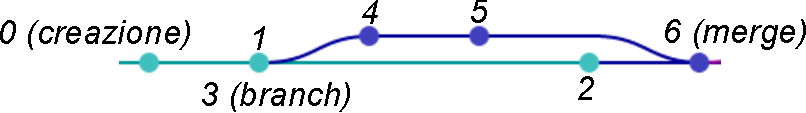
\includegraphics[width=0.99\textwidth]{img/flow0}
}

\subsection{Operazioni preliminari}

\fr{Installazione e configurazione}{
	\bl{In generale}{
		Come ogni prodotto software, i DVCS necessitano di alcune operazioni di configurazione preliminari. In particolare, richiedono di impostare un nome utente ed una email (in modo da poter capire chi ha apportato modifiche e contattarlo).
	}
	\bl{In Mercurial}{
		Mercurial gestisce la configurazione nel file \texttt{\textbf{hgrc}} posizionato nella home directory
		\iz {
			\item Su *nix: \texttt{\textasciitilde{}/.hgrc}
			\item Su Windows: \texttt{\%USERPROFILE\%\textbackslash{}Mercurial.ini}
			\item Istruzioni per la configurazione: \url{http://mercurial.selenic.com/wiki/QuickStart}
		}
		\scriptsize \alert{Utenti windows}: fate attenzione all'estensione del file. Molti software Windows, incluso il file manager, hanno l'abitudine di apporre una loro estensione di default. Fate attenzione a creare \texttt{Mercurial.ini} e non \texttt{Mercurial.ini.txt} (verificate il nome del file con il terminale).
	}
}

\begin{frame}[fragile]{Il file \textbf{hgrc}}
	\begin{itemize}
		\item Comincia con \texttt{[ui]}, che identifica l'inizio dell'omonima sezione
		\item In molti casi, è sufficiente una sola riga di configurazione, con username ed email
		\item Opzionalmente, è possibile specificare un editor
	\end{itemize}
	\begin{block}{Esempio}
		\begin{verbatim}
			[ui]
			username = Danilo Pianini <danilo.pianini@unibo.it>
			editor = kwrite
		\end{verbatim}
	\end{block}
	\scriptsize \alert{Utenti MacOS X}: di default Mercurial su MacOS X utilizza \texttt{vi} come editor. A meno che non lo conosciate, specificate \texttt{nano} o il percorso completo verso l'eseguibile di un editor di testo di vostro gradimento.
	
	\alert{Utenti Linux}: di default Mercurial \textbf{dovrebbe} usare \texttt{nano} come editor. Visto che ciascuna distribuzione potrebbe comportarsi diversamente, è comunque bene specificare il comando del vostro editor preferito (ad esempio \texttt{nano}) - eventualmente anche con gui (ad esempio \texttt{gedit}).

\end{frame}

\subsection{Operazioni di base sul repository}

\fr{Inizializzazione}{
	\bl{In generale}{
		È necessario esplicitare che, da un certo punto del file system, si desidera utilizzare il DVCS per tener traccia dei cambiamenti dei file contenuti da quel punto in poi.
	}
	\bl{In Mercurial}{
		\iz{
			\item \texttt{hg init}
		}
		Marca la cartella corrente come repository Mercurial. Crea una sottocartella nascosta \texttt{.hg} nella quale saranno salvati i metadati. Fintanto che la cartella \texttt{.hg} è integra, sarà possibile ripristinare lo stato dei file del repository a qualunque versione. Il file \texttt{.hg/hgrc} può contenere impostazioni che sovrascrivono (per il repository locale) quelle di \texttt{\textasciitilde{}/.hgrc}. Il formato del file è lo stesso di \texttt{\textasciitilde{}/.hgrc}.
	}
}

\fr{Aggiunta}{
	\bl{In generale}{
		È necessario segnalare esplicitamente quali file si vogliono tracciare. La ragione è che molti dei file potrebbero essere rigenerabili a partire da altri, si pensi ad esempio ai file binari che possono essere ricompilati a partire dai sorgenti: tracciarli è un inutile dispendio di risorse!

		Il tracking differenziale è molto efficiente e veloce nel tracking di file di testo, mentre è \textbf{molto inefficiente} nel tracciare file binari. La regola è quindi quella di tracciare solo e soltanto i files non rigenerabili. Nel caso di un progetto Java, esclusivamente i sorgenti (\texttt{*.java}) e le eventuali risorse (icone, XML, etc.). \textbf{Mai} tracciare \texttt{class} files o documentazione rigenerabile (Javadoc).
	}
	\bl{Esempi con Mercurial}{
		\iz{
			\item \texttt{hg add nomefile1 nomefile2 directory1 directory2}
			\item \texttt{hg add *}
		}
	}
}

\fr{Ignorare files} {
	\bl{In generale} {
		Dato che spesso si vogliono aggiungere moltissimi file con un solo comando evitando di elencarli, è necessario offrire un meccanismo che consenta di descrivere quali file si vogliono tracciare ed escluderne automaticamente altri.

		È anche un'ottima pratica per evitare possibili errori!
	}
	\bl{In Mercurial}{
		\iz{
			\item È possibile creare un file \texttt{.hgignore} che contenga informazioni circa i file da ignorare.
			\item È possibile utilizzare una sintassi classica (\texttt{glob}, consigliata) oppure una sintassi avanzata (basata su regular expressions).
		}
	}
}

\begin{frame}[fragile]{Il file \texttt{.hgignore}}
	\begin{block}{Esempio di contenuto del file}
		\scriptsize
		\begin{verbatim}
		syntax: glob
		*.class
		*_gen
		*_trace
		*/target/*
		*hs_err_pid*
		*/bin/*
		\end{verbatim}
	\end{block}
	\begin{block}{Il file così scritto ignora:}
		\begin{itemize}
			\item Tutti i files il cui nome termina in \texttt{.class}
			\item Tutti i files il cui nome termina in \texttt{\_gen}
			\item Tutti i files il cui nome termina in \texttt{\_trace}
			\item Tutti i files il cui path completo contenga una cartella di nome \texttt{target} 
			\item Tutti i files nel cui path completo compaia a qualunque punto la stringa \texttt{hs\_err\_pid} 
			\item Tutti i files il cui path completo contenga una cartella di nome \texttt{bin} 
		\end{itemize}
	\end{block}
\end{frame}


\fr{Rimozione}{
	\bl{In generale}{
		Come l'aggiunta, la rimozione deve essere esplicita. Quando si rimuove un file tracciato, infatti, vi sono due opzioni:
		\begin{enumerate}
			\item Si desidera rimuovere il file, registrarne la rimozione e cessare di farne il tracking (se venisse ricreato, andrebbe riaggiunto). È l'opzione più comune.
			\item Si desidera rimuovere il file dalla working copy, ma si desidera mantenere l'ultima versione del file come tracciato.
		\end{enumerate}
		Se si desidera la prima opzione, è necessario segnalarlo al DVCS.
	}
	\bl{In Mercurial}{
		\iz{
			\item \texttt{hg rm file1 file2}
		}
		Rimuove \texttt{file1} e \texttt{file2} dalla working copy e registra il fatto che sono stati rimossi (se ricreati, andranno riaggiunti con \texttt{hg add}).
	}
}

\fr{Rinominazione}{
	\bl{In generale}{
		La rinominazione può essere vista come una rimozione e una riaggiunta, per cui presenta gli stessi problemi della rimozione.

		Se si desidera (normalmente è così) far sì che il DVCS registri il cambio di nome di un file, è necessario eseguirlo esplicitamente.
	}
	\bl{In Mercurial}{
		\iz{
			\item \texttt{hg mv file1 file2}
		}
		Rinomina \texttt{file1} in \texttt{file2} nella working copy e registra il fatto che \texttt{file1} è stato rimosso e \texttt{file2} è stato aggiunto al tracking.
	}
}

\subsection{Stato corrente, commit e diff}

\fr{Stato}{
	\bl{In generale}{
		È necessario avere la possibilità di capire in qualunque momento quali file nel repository sono stati modificati, quali rimossi e quali sono nuovi
	}
	\bl{In Mercurial}{
		\iz{
			\item \texttt{hg status}
		}
		Produce un elenco di file il cui stato non è lo stesso della revision attiva di Mercurial. Ognuno è preceduto da una lettera indicante perché differisce:
		\iz{
			\item \texttt{M} --- File modificato rispetto alla versione corrente
			\item \texttt{A} --- File aggiunto (con \texttt{hg add})
			\item \texttt{R} --- File rimosso (con \texttt{hg rm})
			\item \texttt{!} --- File rimosso manualmente ma ancora tracciato
			\item \texttt{?} --- File non tracciato e non ignorato
		}
	}
}

\fr{Salvataggio}{
	\bl{In generale}{
		È necessario avere una operazione che segnali al DVCS che intendiamo eseguire uno snapshot (commit) dello stato corrente di alcuni dei file, generando una nuova versione.

		Assieme con lo stato dei file, vengono automaticamente salvati:
		\iz{
			\item L'utente che ha eseguito il commit e la sua email
			\item Un messaggio di commit. \textbf{È estremamamente importante che il messaggio di commit sia sensato.}
		}
	}
}

\fr{Salvataggio}{
	\bl{In Mercurial}{
		\iz{
			\item \texttt{hg commit file1 file2 file3} --- Crea una nuova revision contenente la versione corrente di \texttt{file1}, \texttt{file2} e \texttt{file3} (se con stato \texttt{M}, \texttt{A} o \texttt{R} in \texttt{hg status}). Viene aperto un editor di testo per l'inserimento del commit message.
			\item \texttt{hg commit} --- Crea una nuova revision contenente la versione corrente di tutti i file modificati o rimossi (stato \texttt{M}, \texttt{A} o \texttt{R} in \texttt{hg status}) Viene aperto un editor di testo per l'inserimento del commit message.
			\item \texttt{hg commit GraphImpl.java -m \ditto{}Improve efficiency of getPath()\ditto{}} --- Crea una nuova revision contenente la versione corrente di \texttt{GraphImpl.java}. Il messaggio di commit sarà \texttt{Improve efficiency of getPath()}.
		}
	}
}

\fr{Diff}{
	\bl{In generale}{
		Come detto, i DVCS utilizzano il tracking differenziale, ossia invece di salvare una copia di ciascun file salvano l'insieme di modifiche necessario a generare i nuovi files a partire dai file precedenti.

		È necessario uno strumento che consenta di visualizzare quali sono le modifiche che saranno apportate ad un certo file
	}
	\bl{In Mercurial}{
		\scriptsize
		\iz{
			\item \texttt{hg diff}
			\item \texttt{hg diff file}
			\item \texttt{hg diff -r RN1 -r RN2 file}
		}
		Mostra su schermo quali differenze saranno salvate al momento del commit in formato standard (lo stesso del comando UNIX \texttt{diff}). L'output è interpretabile dal comando \texttt{diff} e può essere utilizzato per creare delle ``patch''. È possibile specificare il nome dei file che si vuole visualizzare e il numero delle revision che si vogliono confrontare.
	}
}

\begin{frame}[fragile]{Esempio di output del comando \texttt{hg diff}}
\scriptsize
\begin{verbatim}
danysk@apiceworkstation ~ $ hg diff -r 2075 -r 2080 EnvironmentBuilder.java
diff -r e37f2d9e346c EnvironmentBuilder.java
--- EnvironmentBuilder.java    Thu Oct 16 12:23:56 2014 +0200
+++ EnvironmentBuilder.java    Fri Nov 07 15:43:45 2014 +0100
@@ -99,7 +99,9 @@
              final String args = son.getNodeValue();
 //           final StringTokenizer tk = new StringTokenizer(args, " ,;");
              final ArrayList<String> arguments = new ArrayList<String>(1);
-             arguments.add(args);
+             if(!args.isEmpty()) {
+                 arguments.add(args);
+             }
 //           while (tk.hasMoreElements()) {
 //               arguments.add(tk.nextToken());
 //           }

\end{verbatim}
\end{frame}

\subsection{Gestione della history}

\fr{Log}{
	\bl{In generale}{
		Occorre un comando che consenta di visualizzare l'elenco dei commit, chi li ha effettuati, quando, e quali sono le differenze dall'uno all'altro.
	}
	\bl{In Mercurial}{
		\iz{
			\item \texttt{hg log}
			\item \texttt{hg log --limit 10}
		}
		Mostra su standard output la lista di tutti commit. L'opzione \texttt{--limit N} limita il numero di commit visualizzati agli ultimi \texttt{N}.
	}
}

\fr{Log}{
	\bl{In Mercurial}{
		Informazioni del log:
		\iz{
			\item \texttt{changeset} --- Il numero del salvataggio, seguito da un codice hash univoco
			\item \texttt{tag} [OPZIONALE] --- Eventuale nome tag associato al changeset
			\item \texttt{parent} [OPZIONALE] --- Il changeset del salvataggio precedente. Se si tratta di un merge commit, i parent sono almeno due
			\item \texttt{user} --- L'utente che ha eseguito il commit e la sua email
			\item \texttt{date} --- La data in cui il commit è stato registrato
			\item \texttt{summary} --- Il commit message
			\item Utilizzando l'opzione \texttt{-G} --- Visualizzazione grafica delle linee di sviluppo
		}
	}
}

\begin{frame}[fragile]{Esempio di output del comando \texttt{hg log}}
\scriptsize
\begin{verbatim}
danysk@apiceworkstation ~/Dropbox/Alchemist/Alchemist $ hg log --limit 3
changeset:   2081:e37f2d9e346c
tag:         tip
parent:      2067:8f158282ebea
parent:      2080:ad571bda2cc6
user:        Danilo Pianini <danilo.pianini@unibo.it>
date:        Thu Oct 16 12:23:56 2014 +0200
summary:     Merged in smontagna/alchemist-bio (pull request #64)

changeset:   2080:ad571bda2cc6
user:        Sara Montagna <sara.montagna@unibo.it>
date:        Tue Oct 14 11:33:35 2014 +0200
summary:     Fix code (for intracellular simulation) according to FindBugs and PMD rules

changeset:   2079:5bc295d59fbf
user:        Sara Montagna <sara.montagna@unibo.it>
date:        Mon Oct 13 11:41:32 2014 +0200
summary:     fix a bug on ChangeBiomolConcentrationInCell

\end{verbatim}
\end{frame}

\fr{Update}{
	\bl{In generale}{
		Abbiamo una lista di commit, dobbiamo essere in grado di navigarla aggiornando i file tracciati alla revision desiderata.

		Esiste una funzionalità che consente di andare avanti e indietro nella history.
	}
	\bl{In Mercurial}{
		\iz{
			\item \texttt{hg update -r RN --clean}
		}
		Aggiorna tutti i file del repository alla revision \texttt{RN}. L'opzione \texttt{--clean} forza l'aggiornamento dei file e \textbf{scarta tutte le modifiche} che non sono state soggette ad un \texttt{commit}.
	}
}

\subsection{Branching}

\begin{frame}{Branching}
	\begin{block}{Il concetto di branching}
		Dal momento in cui possiamo andare indietro nella storia ed effettuare nuovi commit, abbiamo la possibilità di fare \textit{branching}: abbiamo più di una linea di sviluppo che viene portata avanti!
		\begin{center}
			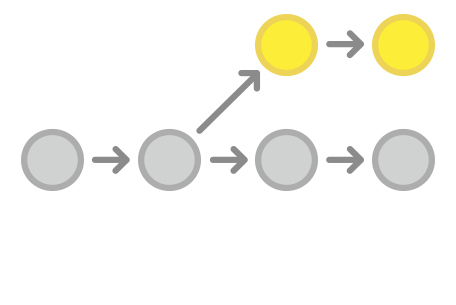
\includegraphics[width=0.6\textwidth]{img/branch}
		\end{center}
	\end{block}
\end{frame}

\begin{frame}{Branching esplicito vs. implicito}
	In Mercurial, a seconda che si dia o meno un nuovo nome al branch, è possibile che:
	\begin{enumerate}
		\item Si avvii una nuova linea di sviluppo senza dichiararla. In questo caso, Mercurial tratta la situazione come \textbf{un singolo branch con più teste di sviluppo}. È una situazione che si vuole evitare, nel caso in cui accada si vuole sempre riunire le teste in una unica (merge). \\ \alert{Nota}: git proibisce espressamente questo genere di branching
		\item Si dichiara che si sta avviando una nuova linea di sviluppo e le si dà un nome. Viene creato un cosiddetto ``named branch'', il DVCS offre comandi che supportano la creazione di più linee ed il passaggio da una all'altra.
	\end{enumerate}
\end{frame}

\begin{frame}{Branching implicito: visualizzazione delle teste}
	Dal momento in cui possiamo andare indietro nella storia ed effettuare nuovi commit, abbiamo la possibilità di fare \textit{branching implicito}: potremmo trovarci nella situazione di avere più teste! C'è la necessità di vedere quante sono e a che punto sono.
	\begin{center}
		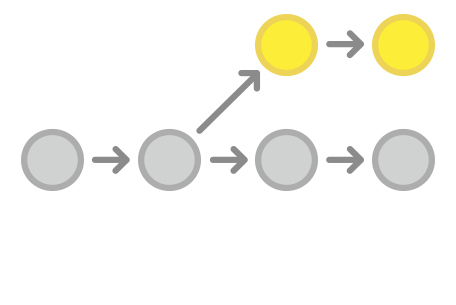
\includegraphics[width=0.6\textwidth]{img/branch}
	\end{center}
	\bl{In Mercurial}{
		\iz{
			\item \texttt{hg heads}
		}
		Mostra tutte le linee di sviluppo attualmente attive (l'output è simile a quello di \texttt{hg log}).
	}
\end{frame}

\begin{frame}{Branching esplicito}
	Per la gestione dei named branches occorrono una serie di strumenti:
	\begin{itemize}
		\item Visualizzazione del branch corrente
		\item Creazione di un nuovo branch
% 		\item Chiusira di un branch non più usato, ad esempio perché è stato usato per sviluppare una nuova feature, ed ora la feature è pronta per essere inserita nella linea di sviluppo principale.
		\item Passaggio ad un altro branch
		\item Merge di due branch
	\end{itemize}
\end{frame}

\begin{frame}{Branching: operazioni di base}
	\begin{block}{Visualizzare il branch corrente}
		\begin{center}
			\texttt{hg branch}
		\end{center}
		Visualizza il nome del branch corrente. Se non si è creato alcun branch manualmente, esiste un solo branch chiamato \texttt{default}
	\end{block}
	\begin{block}{Creazione di un nuovo branch}
		\begin{center}
			\texttt{hg branch nome\_del\_nuovo\_branch}
		\end{center}
		Assegna il nome \texttt{nome\_del\_nuovo\_branch} al branch corrente: a partire dal commit successivo, si lavorerà su \texttt{nome\_del\_nuovo\_branch}
	\end{block}
	\begin{block}{Passaggio ad un altro branch}
		\begin{center}
			\texttt{hg update nome\_del\_branch}
		\end{center}
		Assegna il nome \texttt{nome\_del\_nuovo\_branch} al branch corrente: a partire dal commit successivo, si lavorerà su \texttt{nome\_del\_nuovo\_branch}
	\end{block}
\end{frame}


\fr{Merge}{
	\bl{In generale}{
		Dal momento in cui possiamo avere più branch, oppure un branch con più teste, abbiamo necessità di uno strumento che ci consenta di riunirle. Ad esempio:
		\begin{itemize}
			\item Abbiamo creato un nuovo branch per testare una nuova feature senza danneggiare il nostro software funzionante. Ora tutto è a posto, e vogliamo integrare le modifiche nella ``mainline''
			\item Siamo andati indietro nella storia, abbiamo visto un errore e l'abbiamo corretto senza fare un nuovo branch. Dopo il commit, ci troviamo un branch con due teste, e vogliamo riunirle.
		\end{itemize}
		\begin{center}
			\centering{}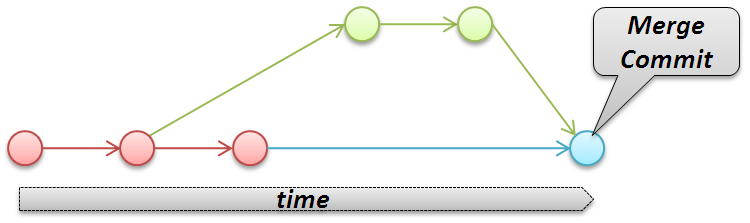
\includegraphics[width=0.6\textwidth]{img/merge}
		\end{center}
	}
}

\begin{frame}{Merge di più teste in Mercurial}
	Nel caso in cui vi siano più teste nel branch corrente, il comando
	\begin{center}
		\texttt{hg merge}
	\end{center}
	Tenta di unirle.
	Una volta che il merge è completo, per registrare le modifiche è necessario eseguire un \texttt{commit}.

	Grazie al tracciamento differenziale, esistono algoritmi molto potenti che consentono di risolvere automaticamente la maggior parte dei conflitti. È comunque possibile che, in caso di modifiche sullo stesso file, si generi un \emph{conflitto di merge}. Quando capita, il conflitto andrà risolto manualmente.
\end{frame}

\begin{frame}{Merge di più branch in Mercurial}
	Nel caso di più branch, si fa un'operazione analoga. Supponiamo di avere due branch: uno chiamato \texttt{mainline}, dove teniamo lo sviluppo principale, ed uno chiamato \texttt{feature}, dove abbiamo sviluppato una nuova funzionalità che adesso vogliamo portare sul nostro branch principale.
	\begin{enumerate}
	 \item Si passa al branch ``destinazione'', ossia quello che consideriamo essere il principale. Se si è già nel branch corretto, e se non ci sono modifiche pendenti, non è necessario.
		\begin{itemize}
			\item \texttt{hg update mainline --clean}
		\end{itemize}
	 \item Si fa il merge del branch che contiene le nuove feature in modo analogo a quello che abbiamo fatto nel caso di più teste:
		\begin{itemize}
			\item \texttt{hg merge feature}
			\item \texttt{hg commit -m "Merge feature into mainline"}
		\end{itemize}
	 \item Si segnala che il branch precedente non sarà più usato ``chiudendolo'' con uno speciale commit:
		\begin{itemize}
			\item \texttt{hg update feature}
			\item \texttt{hg commit --close-branch -m "Close branch feature"}
			\item \texttt{hg update mainline}
		\end{itemize}
	\end{enumerate}
\end{frame}

% \fr{Esercizio con Mercurial}{
% 	Tenendo a mente quanto spiegato finora e facendo uso delle informazioni nelle slides precedenti, svolgere \textbf{in ordine} i seguenti punti.
% 	\iz {
% 		\item Si configuri Mercurial, creando il file di configurazione appropriato a seconda che si stia usando un sistema *nix o Windows
% 		\item Si apra un terminale
% 		\item Si crei una nuova cartella
% 		\item Ci si posizioni col terminale nella nuova cartella
% 		\item Si inizializzi un nuovo repository Mercurial
% 		\item Si crei, utilizzando un editor di testo (e.g. JEdit) un file \texttt{HelloWorld.java}, che contenga una sola classe \texttt{HelloWorld} ed un metodo main con una sola \texttt{println}
% 		\item Si aggiunga \texttt{HelloWorld.java} al repository
% 		\item Si osservi lo stato del repository con \texttt{hg status}
% 		\item Si effettui il primo commit, inserendo un commit message sensato (ad esempio ``create new HelloWorld class''), senza utilizzare l'opzione \texttt{-m}
% 	}
% }
% 
% \fr{Esercizio con Mercurial}{
% 	\iz {
% 		\item Si osservi nuovamente lo stato del repository con \texttt{hg status}
% 		\item Si osservi la history dei commit utilizzando \texttt{hg log}
% 		\item Si modifichi \texttt{HelloWorld.java}, cambiando la stringa che viene stampata nella \texttt{println}
% 		\item Si osservi nuovamente lo stato del repository con \texttt{hg status}
% 		\item Si osservi la modifica fatta al file \texttt{HelloWorld.java} utilizzando propriamente \texttt{hg diff}
% 		\item Si faccia il commit delle modifiche, stavolta utilizzando l'opzione \texttt{-m}
% 		\item Si compili nella cartella \texttt{bin} il file HelloWorld.java
% 		\item Si osservi nuovamente lo stato del repository con \texttt{hg status}. Si noti che Mercurial rileva dei nuovi file che non sono ancora tracciati
% 	}
% }
% 
% \fr{Esercizio con Mercurial}{
% 	\iz {
% 		\item Dato che non desideriamo tracciare file che possono essere compilati, si scriva un file \texttt{.hgignore} che faccia sì che Mercurial ignori tutti i file con estensione \texttt{.class} e tutti i file nel cui path è presente una cartella chiamata \texttt{bin}
% 		\item Si verifichi con \texttt{hg status} che il file compilato non viene più mostrato fra quelli tracciabili, mentre viene mostrato \texttt{.hgignore}
% 		\item Si aggiunga \texttt{.hgignore} al tracker e si faccia commit
% 		\item Modificare \texttt{HelloWorld.java} in modo tale che non compili. Assicurarsi che non compili utilizzando \texttt{javac}
% 		\item Correggere l'errore inserito facendo roll back con \texttt{hg update --clean}
% 		\item Verificare con \texttt{hg status} che il repository sia stato portato allo stato precedente, quindi compilarlo con \texttt{javac}
% 		\item Tornare al primo commit effettuato con \texttt{hg update -r0 --clean}
% 		\item Ricompilare ed eseguire, verificando che si sia tornati allo stato iniziale
% 	}
% }
% 
% \fr{Esercizio con Mercurial}{
% 	\iz {
% 		\item Creare un nuovo file \texttt{readme.txt} utilizzando un editor di testo. Inserire al suo interno nome, cognome e matricola.
% 		\item Si aggiunga \texttt{readme.txt} al tracker
% 		\item Si faccia commit
% 		\item Si rinomini, utilizzando \texttt{hg mv}, \texttt{readme.txt} in \texttt{readme.md}
% 		\item Verificare con \texttt{hg status} quale sia lo stato del repository
% 		\item Si faccia commit della modifica
% 		\item Si osservi, utilizzando \texttt{hg heads}, che si abbiano due linee di sviluppo (in una c'è \texttt{HelloWorld.java} aggiornato e \texttt{.hgignore}, nell'altro il file \texttt{readme.md})
% 		\item Si uniscano le linee di sviluppo con \texttt{hg merge} (se tutto è stato eseguito correttamente, non ci saranno merge conflict)
% 		\item Si esegua il commit dell'operazione di merge
% 		\item Si utilizzi \texttt{hg log} per osservare la storia del repository. Si noti che il commit corrente ha due parent.
% 	}
% }
% 
% \fr{Esercizio con Mercurial}{
% 	\iz {
% 		\item Si cancellino tutti i file dal repository a mano (senza utilizzare \texttt{hg rm}, ma semplicemente rimuovendoli)
% 		\item Si osservi lo stato del repository con \texttt{hg status}
% 		\item Si ripristini i file cancellati con \texttt{hg update --clean}
% 		\item Si rimuova dal tracking il file \texttt{readme.md} utilizzando \texttt{hg rm}
% 		\item Si faccia il commit della modifica
% 		\item Utilizzando hg log, si osservi tutta la storia del repository, quindi si visualizzino solo le ultime due operazioni.
% 	}
% }

\begin{frame}{Esercizio}
	Provate a svolgere l'esercizio 0 dell'esercitazione. Troverete un file di istruzioni che vi spiegherà dettagliatamente il da farsi.
\end{frame}


\fr{Nella prossima puntata}{
	\iz {
		\item Merge conflicts e loro risoluzione
		\item Servizi di hosting per repository Mercurial e Git
		\item Lavoro parallelo in gruppo con DVCS
		\item Aspetti avanzati: rebasing, bisection, cherry picking (cenni)
		\item Workflow suggeriti per sfruttare al massimo i DVCS
		\item Il menù ``Team'' di Eclipse e il plug-in HGE
	}
}

\section{Lab Startup}

\fr{Preparazione Ambiente di Lavoro 1/2}{
	\iz{
		\item Accendere il PC
		\item Loggarsi sul sito del corso
		\iz{
			\item \textcolor{blue}{\url{https://elearning-cds.unibo.it/course/view.php?id=3042}}
		}
		\item Scaricare dalla sezione \texttt{lab} del sito il file \texttt{oop1415-lab07.zip} contenente il materiale dell'esercitazione odierna
		\item Spostare il file scaricato sul Desktop
		\item Decomprimere il file usando 7zip (o un programma analogo) sul Desktop
	}
}

\fr{Preparazione Ambiente di Lavoro 2/2}{
	\iz{
		\item Copiare la cartella scompattata nel vostro workspace di Eclipse
		\iz{
			\item p.e. \texttt{C:$\backslash$Users$\backslash$<username>$\backslash$workspace}
		}
		\item Importare il progetto \texttt{OOP1415\_Lab07\_Code} con la procedura standard di importazione dei progetti
	}
}


\fr{Modalità di Lavoro}{
  \bl{}{
    \en{
      \item Gli esercizi sono divisi in package con nomi progressivi
      \item Troverete un commento con le istruzioni per ciascun esercizio
      \item Risolvere l'esercizio in autonomia
      \item Cercare di risolvere autonomamente eventuali piccoli problemi che possono verificarsi durante lo svolgimento degli esercizi
      \item \textcolor{red}{Utilizzare i test JUnit presenti nei sorgenti per il testing dell'esercizio}
      \item Contattare i docenti nel caso vi troviate a lungo bloccati nella risoluzione di uno specifico esercizio
      \item \textbf{A esercizio ultimato contattare i docenti per un rapido controllo della soluzione realizzata}
      \item Proseguire con l'esercizio seguente
    }
  }
}
\end{document}

%%%%%%%%%%%%%%%%%%%%%%%%%%%%%%%%%%%%%%
%%%% TO BE REUSED ON NEXT LAB %%%%%%%%
%%%%%%%%%%%%%%%%%%%%%%%%%%%%%%%%%%%%%%

\subsection{Lavorare con più repository}

\fr{Clone}{
  Esiste ovviamente la possibilità di clonare un repository già esistente, sul quale volete lavorare.\\
  \bl{il comando \texttt{clone}}{
    \texttt{clone} deve essere seguito dall'URI a cui si trova il repository che volete clonare. Può essere un repository sul vostro disco, può essere un repository che si trova online (vedremo dopo alcuni servizi di hosting), può essere un repository che si trova nella vostra rete locale.
  }
  \bl{Esempi}{
    \iz{
      \item \texttt{clone /home/user/repo1 /home/user/repo2} --- Clona un repository sul disco locale nel path specificato.
      \item \texttt{clone https://user@service.org/repo /home/user/repo2} --- Clona un repository remoto sul disco, nel path specificato, con protocollo HTTPS.
    }
    Si noti che gli URI da inserire in clone possono essere DVCS-specifici.
  }
}

\fr{Pull}{
  L'operazione di \texttt{pull} consente di prendere dati da un altro repository per inserirli nel proprio.\\
  \bl{il comando \texttt{pull}}{
    \texttt{clone} deve essere seguito dall'URI a cui si trova il repository di cui volete copiare le differenze. Ovviamente, i due repository devono avere la stessa radice, ossia avere una parte in comune.
  }
}

\fr{Push}{
  \bl{In teoria, l'operazione di \texttt{pull} è sufficiente. In pratica, no.}{
    \iz {
      \item Se il repository locale è su una macchina NATtata?
      \item Se il repository remoto è un server cui non potete accedere per fare \texttt{pull}?
    }
    Serve un meccanismo per ``spingere'' le modifiche verso un altro repository, ossia il complementare di \texttt{pull}. Tale meccanismo è \texttt{push}.
  }
}

\fr{Lavorare in parallelo}{
  \bl{Fin qui tutto molto carino...} {
   ...ma abbiamo lavorato sequenzialmente, e mai in parallelo.
  }
  Il vero vantaggio nell'uso di DVCS si ha quando si comincia a lavorare parallelamente sulla stessa cosa. 
}

\fr{Lavorare in parallelo: esempio}{
  Situazione iniziale:
  \begin{center}
    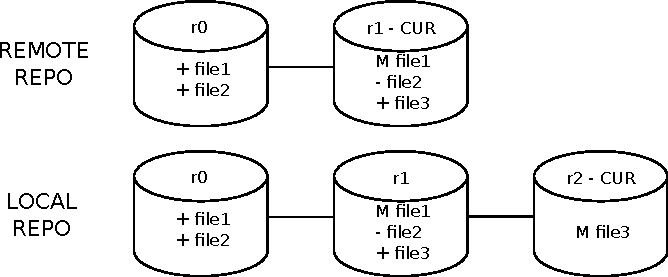
\includegraphics[width=0.99\textwidth]{img/draw5}
  \end{center}
}

\fr{Lavorare in parallelo: esempio}{
  Remote esegue:\\
  Modifica di \texttt{file2} \\
  \texttt{commit} \\
  \begin{center}
    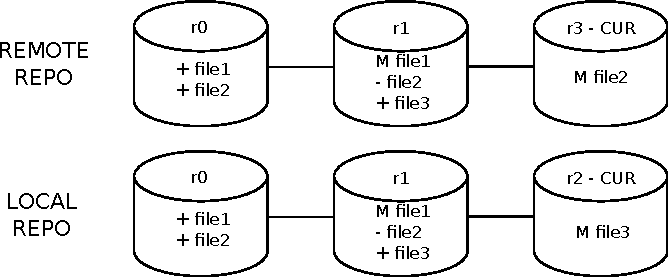
\includegraphics[width=0.99\textwidth]{img/draw7}
  \end{center}
}

\fr{Lavorare in parallelo: esempio}{
  Local esegue:\\
  \texttt{push indirizzo\_di\_remote\_repo} \\
  \texttt{commit} \\
  \begin{center}
    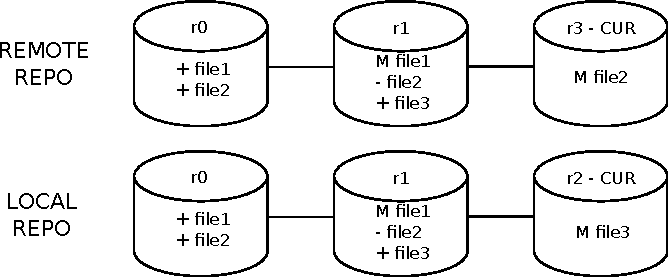
\includegraphics[width=0.99\textwidth]{img/draw7}
  \end{center}
  La push viene rifiutata: la radice dei due repository è diversa!
}

\fr{Lavorare in parallelo: esempio}{
  Local esegue:\\
  \texttt{push indirizzo\_di\_remote\_repo} \\
  \texttt{commit} \\
  \begin{center}
    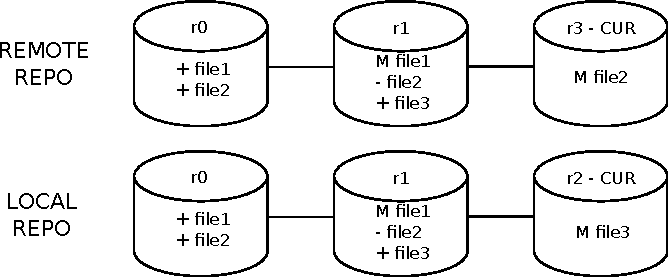
\includegraphics[width=0.99\textwidth]{img/draw7}
  \end{center}
  La push viene rifiutata: la radice dei due repository è diversa!
}

\fr{Lavorare in parallelo: esempio}{
  Local esegue:\\
  \texttt{pull indirizzo\_di\_remote\_repo} \\
  \begin{center}
    \includegraphics[width=0.7\textwidth]{img/draw8}
  \end{center}
  Il repository locale ora può essere portato anche alla versione \texttt{r3}. Nonostante ciò, le push vengono rifiutate, poiché il repository locale ha due teste!
}

\fr{Merge}{
  L'operazione di \texttt{merge} consente di unire due teste di un repository unendo le loro modifiche.
  \iz {
    \item Se le modifiche effettuate concorrentemente non toccano gli stessi files, tali modifiche sono semplicemente unite insieme.
    \item Se le modifiche toccano gli stessi files in parti diverse. il DVCS fa del suo meglio per cercare di risolvere i conflitti.
    \item Se ci sono conflitti a livello della singola linea di codice, è necessario un intervento manuale: l'utente deve selezionare le righe che vuole mantenere nella versione merged.
  }
}

\fr{Merge: esempio}{
  Situazione iniziale:\\
  \begin{center}
    \includegraphics[width=0.7\textwidth]{img/draw8}
  \end{center}
}

\fr{Merge: esempio}{
  Local esegue:\\
  \texttt{merge} \\
  \begin{center}
    \includegraphics[width=0.99\textwidth]{img/draw9}
  \end{center}
  Ora è possibile effettuare push: c'è una sola testa!
}

\fr{Merge: esempio}{
  Local esegue:\\
  \texttt{push indirizzo\_di\_remote\_repo} \\
  \begin{center}
    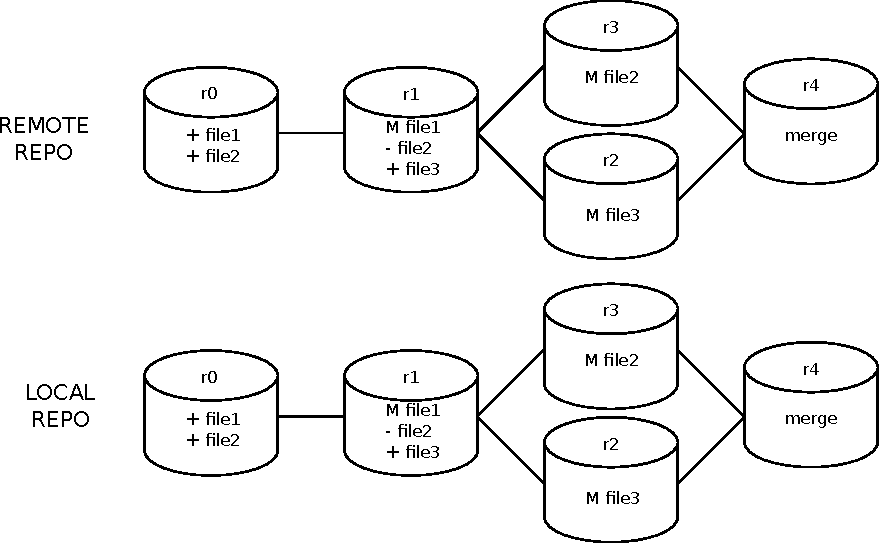
\includegraphics[width=0.8\textwidth]{img/draw10}
  \end{center}
  Ora è possibile effettuare push: c'è una sola testa!
}

\fr{Aspetti avanzati}{
  \bl{Branching}{
    Creazione volontaria di più ``teste''. Si usa, ad esempio, quando si vuole sviluppare una funzionalità sperimentale, e integrarla solo successivamente.
  }
  \bl{Rebasing}{
    Procedura alternativa al merge, in cui i due commit, invece di essere fusi, vengono messi in sequenza.
  }
  \bl{Cherry picking}{
    Pull di un singolo commit. Spesso utilizzato quando si desidera avere un bugfix che si trova in un altro branch, ma non tutto il resto.
  }
  \bl{Bisection}{
    Strategia per scoprire bug in maniera automatizzata, testando il software a varie versioni (ricerca dicotomica). Una volta trovata la prima versione dove il bug si verifica, si controllano commit message e le differenze.
  }
}

\subsection{Un DVCS: Mercurial}

\fr{Plugin Eclipse}{
  È disponibile anche un plugin per Eclipse, che semplifica molto la gestione del repository quando sviluppate con l'IDE.
  \bl{Installazione}{
    \begin{enumerate}
     \item Help $\Rightarrow$ Install new software...
     \item Inserire l'indirizzo \url{http://hge.javaforge.com/mercurialeclipse-snapshots} e premere invio
     \item Selezionare il plugin che viene caricato 
     \item Next
     \item Accettare le eventuali licenze
     \item Accettare l'eventuale richiesta di installazione di software non firmato
     \item Riavviare Eclipse
    \end{enumerate}
  }
}

\fr{Uso del plugin di eclipse}{
  \iz{
    \item   Una volta installato, sarà possibile utilizzare Mercurial dalla veste grafica interna ad Eclipse. I comandi sono accessibili nel sotto-menu ``Team''.
    \item La prima operazione da fare è attivare Mercurial nel progetto, tramite Team $\Rightarrow$ Share. Da questo momento sarà possibile utilizzare tutte le funzioni di Mercurial.
    \item Nota: ricordatevi \textbf{sempre} di mettere correttamente il nome del committer quando eseguite un commit. Il formato è\\ Nome Cognome \textless{}indirizzo@email.qui\textgreater{}
  }
}

\subsection{Servizi di hosting}

\fr{Servizi di hosting}{
  \iz{
    \item Esistono diversi servizi online che vi consentono di mantenere una copia remota del repository
    \item Perché dovreste avere una copia remota?
    \iz{
      \item Sicurezza
      \item Condivisione con altri
      \item Semplificazione dello sviluppo in gruppo
    }
    \item Questi servizi spesso vi forniscono strumenti potenti
    \iz{
      \item Possibilità di visualizzare la storia dello sviluppo
      \item Forks
      \item Pull requests
      \item Commenti per-linea di codice
    }
  }
  I due più comuni sono GitHub (\url{https://github.com/}) e Bitbucket (\url{https://bitbucket.org/}). Il primo supporta solamente git, mentre il secondo supporta sia git che Mercurial.
}

\fr{Bitbucket}{
  \iz {
    \item Vi consigliamo di usare Bitbucket, lo utilizziamo anche noi per le vostre slides e esercitazioni.
    \item Se vi iscrivete utilizzando la mail istituzionale, riceverete un account illimitato gratuitamente (il prezzo dell'account illimitato si aggira sui 120\$ al mese)
  }
}

\fr{Bitbucket: project overview, RSS}{
  \begin{center}
    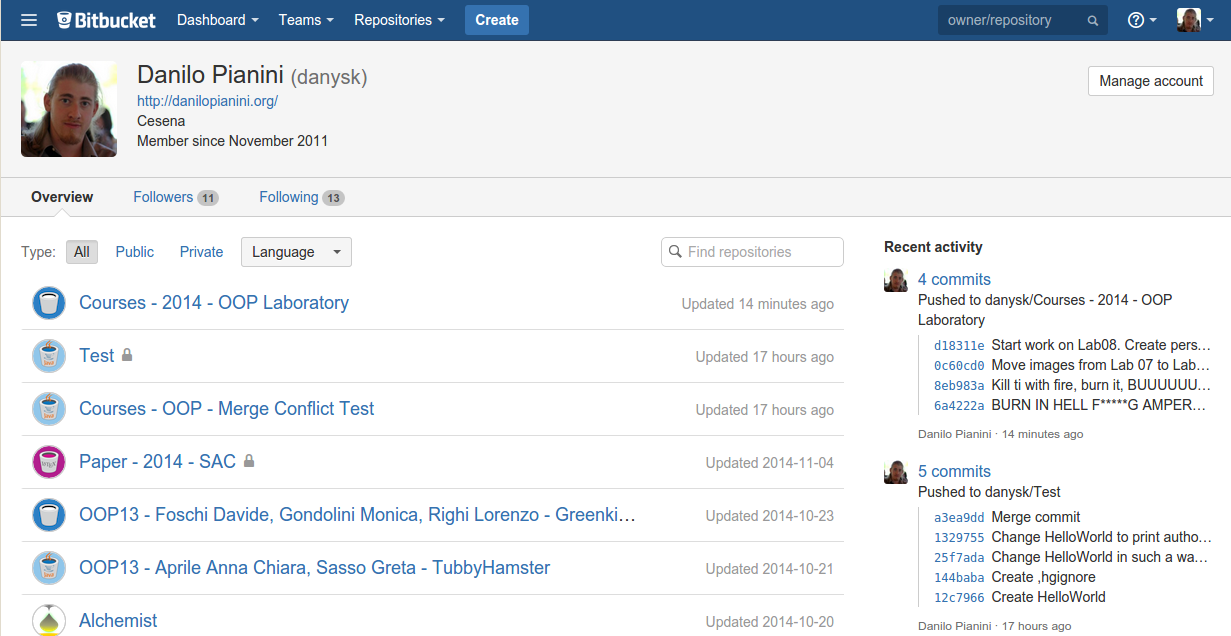
\includegraphics[width=0.99\textwidth]{img/bitbucket0}
  \end{center}
}

\fr{Bitbucket: source navigation}{
  \begin{center}
    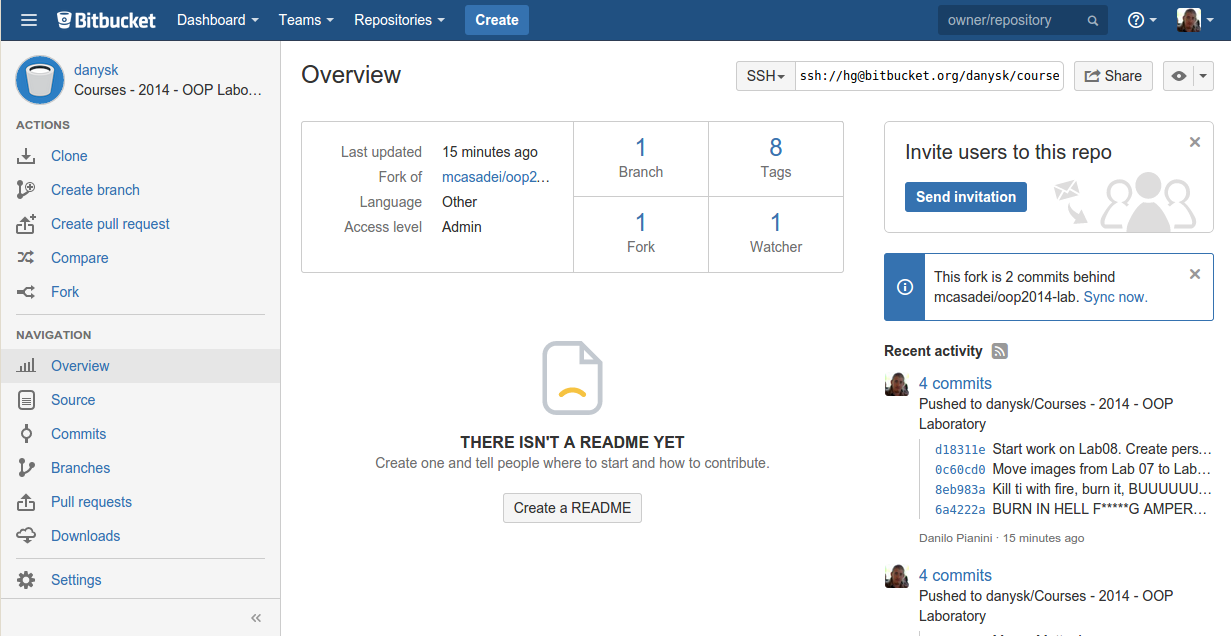
\includegraphics[width=0.99\textwidth]{img/bitbucket1}
  \end{center}
}
\fr{Bitbucket: development history}{
  \begin{center}
    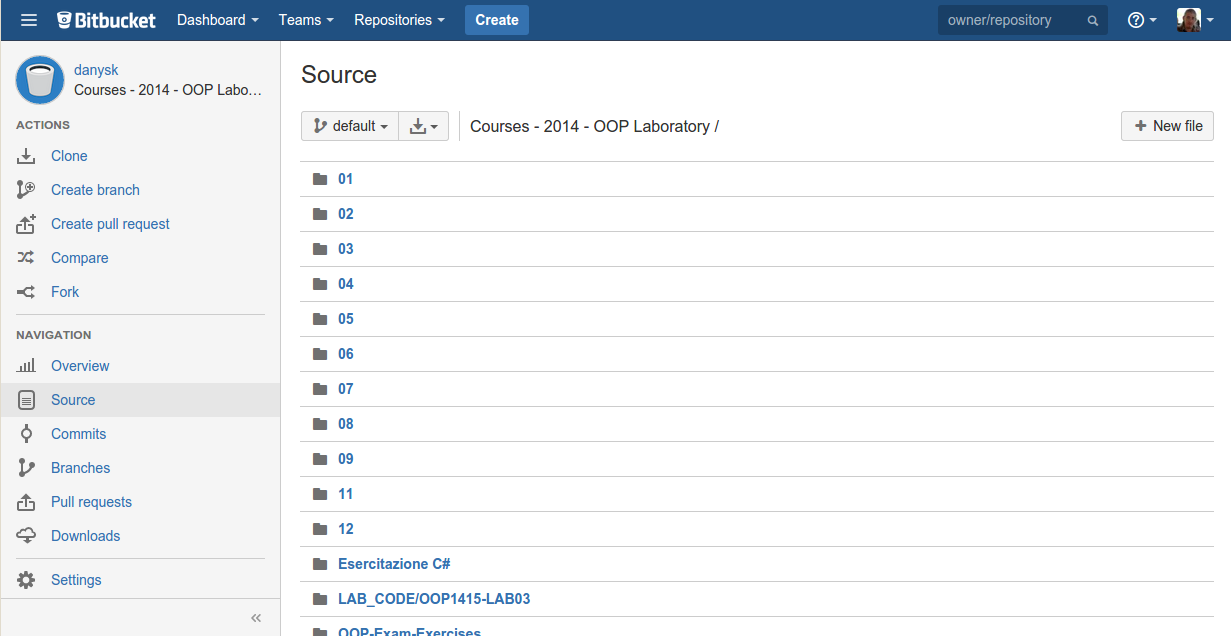
\includegraphics[width=0.99\textwidth]{img/bitbucket2}
  \end{center}
}

\fr{Bitbucket: bug tracker and wiki}{
  \begin{center}
    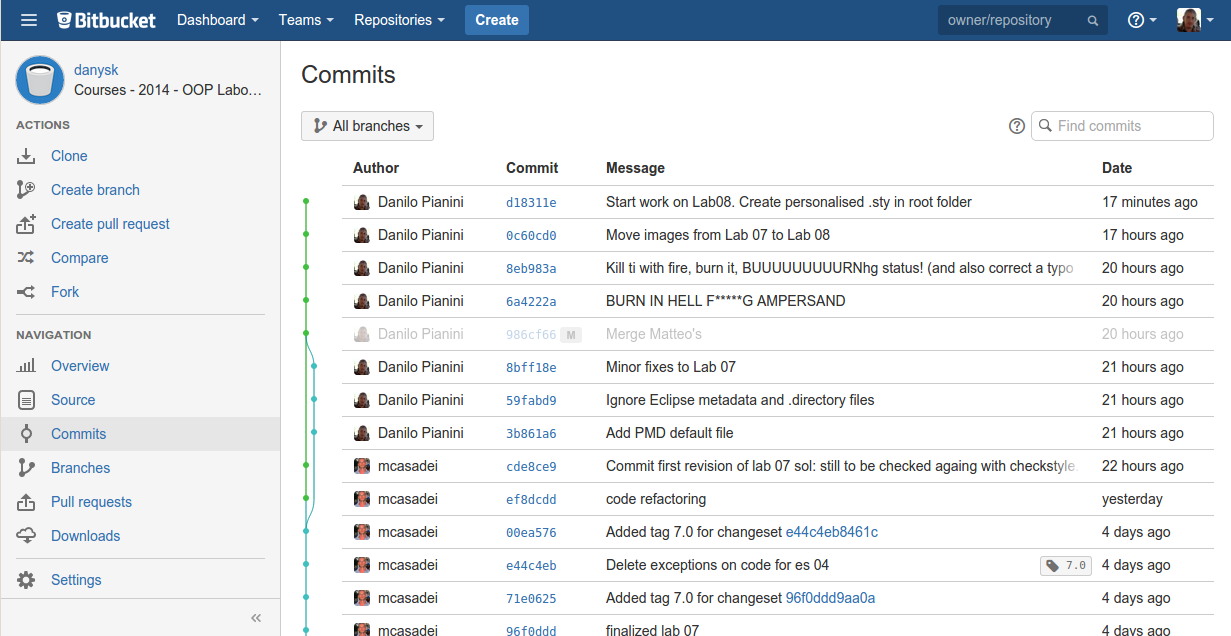
\includegraphics[width=0.99\textwidth]{img/bitbucket3}
  \end{center}
}

\fr{Bitbucket: download page}{
  \begin{center}
    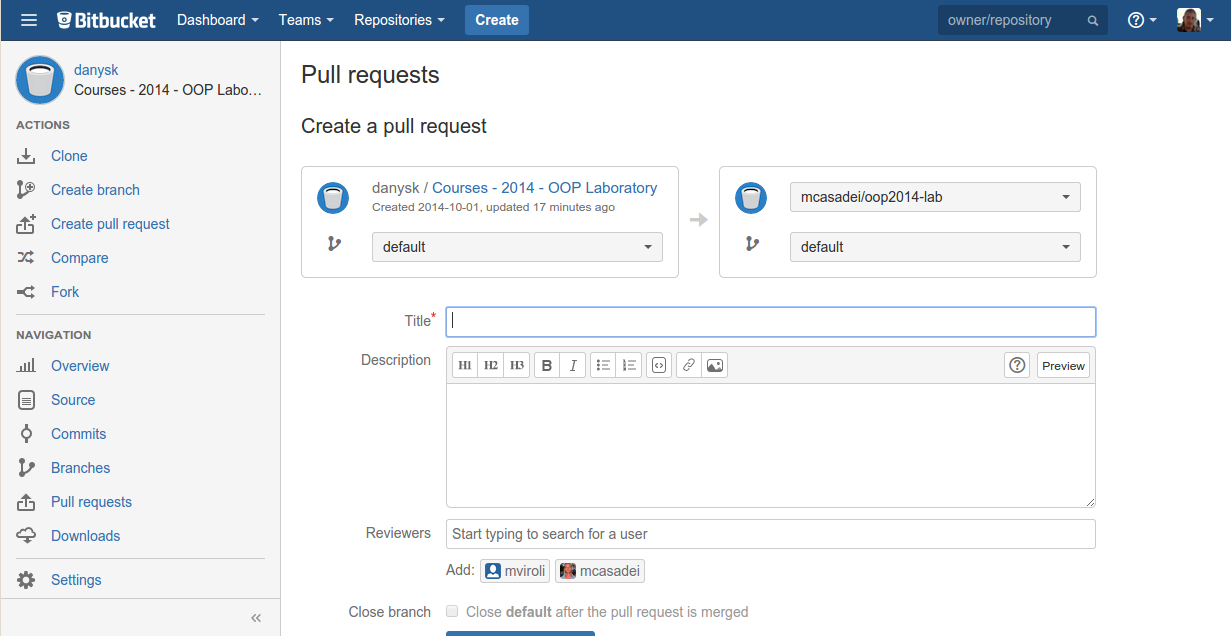
\includegraphics[width=0.99\textwidth]{img/bitbucket4}
  \end{center}
}

\fr{Bitbucket: Pull requests, Compare e Fork}{
  \begin{center}
    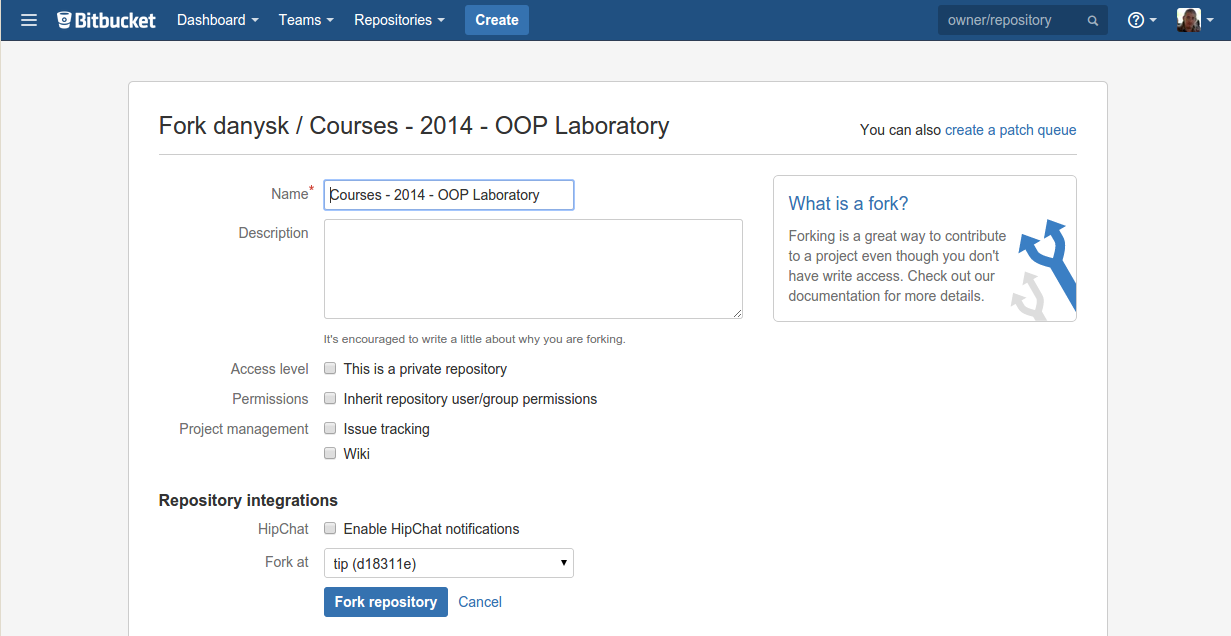
\includegraphics[width=0.99\textwidth]{img/bitbucket5}
  \end{center}
}


\subsection{Workflow suggeriti}
\fr{Esercizio con Mercurial} {
  Utilizzando i comandi visti finora, si svolgano i seguenti passi:
  \begin{enumerate}
   \item Si inizializzi un nuovo repository
   \item Si creino due file di testo e si aggiungano al repository
   \item Si usi \texttt{hg status} per vedere lo stato del repository
   \item Si faccia un commit
   \item Si usi \texttt{hg log} per vedere la storia del repository
   \item Si cancellino i due file dal file system (non dal repository!)
   \item Si ripristinino i due file cancellati sfruttando il comando \texttt{hg update}
   \item Si cloni il repository in un'altra cartella usando \texttt{hg clone}
   \item Si modifichi, nel nuovo repository, uno dei file
   \item Si faccia un commit nel nuovo repository
   \item Si usi \texttt{hg push} per spingere la modifica sul vecchio repository
  \end{enumerate}
  A casa, si facciano ulteriori prove, anche utilizzando il plug-in di Eclipse e creando un repository su Bitbucket. Si sfrutti il forum del corso nel caso si incontrino problemi.
}

